\documentclass{article}

\title{Układy równań liniowych}
\author{Dominik Lau}

\usepackage{blindtext}
\usepackage{amsmath}
\usepackage[utf8]{inputenc}
\usepackage[polish]{babel}
\usepackage[T1]{fontenc}
\usepackage{listings}
\usepackage{color}
\usepackage{amssymb}
\usepackage{esvect}
\usepackage{graphicx}
\usepackage{hyperref}



\definecolor{dkgreen}{rgb}{0,0.6,0}
\definecolor{gray}{rgb}{0.5,0.5,0.5}
\definecolor{mauve}{rgb}{0.58,0,0.82}

\lstset{frame=tb,
  language=Python,
  aboveskip=3mm,
  belowskip=3mm,
  showstringspaces=false,
  columns=flexible,
  basicstyle={\small\ttfamily},
  numbers=none,
  numberstyle=\tiny\color{gray},
  keywordstyle=\color{blue},
  commentstyle=\color{dkgreen},
  stringstyle=\color{mauve},
  breaklines=true,
  breakatwhitespace=true,
  tabsize=3
}
\renewcommand\thesubsection{\Alph{subsection}}
\graphicspath{ {./media/} }

\begin{document}
\maketitle
\section{Wstęp}
Celem projektu była implementacja i przeanalizowanie metod rozwiązywania układów równań liniowych
\begin{gather*}
	\boldsymbol{A}\boldsymbol{x} = \boldsymbol{b}
\end{gather*}
Rozważane metody to metoda faktoryzacji LU, metoda Jacobiego i metoda Gaussa-Seidla.  
Do implementacji wykorzystano język $Python$ oraz bibliotekę $matplotlib$.
\section{Teoria}
\subsection*{Metoda faktoryzacji LU}
Jest to metoda bezpośredniego rozwiązywania układu równań.  Pierw rozbijamy macierz $\textbf{A}$
na dwie macierze trójkątne: dolną $\textbf{L}$ i górną $\textbf{U}$
\begin{gather*}
	\boldsymbol{A} = \boldsymbol{L}\boldsymbol{U}
\end{gather*}
następnie rozwiązujemy dwa układy równań dla macierzy trójkątnych
\begin{gather*}
	\boldsymbol{A}\boldsymbol{x} = \boldsymbol{b}\\
	 \boldsymbol{L} \boldsymbol{U}  \boldsymbol{x} =  \boldsymbol{b} \\
	 \boldsymbol{Ux} =  \boldsymbol{y}  \\\\
	 \boldsymbol{L}  \boldsymbol{y} =   \boldsymbol{b}
\end{gather*}
powyższe równanie rozwiązujemy dla $ \boldsymbol{y}$, następnie rozwiązujemy dla $\boldsymbol{x}$
korzystając z zależności
\begin{gather*}
	\boldsymbol{Ux} =  \boldsymbol{y}  \\\\
\end{gather*}
\subsection*{Metoda Jacobiego}
Jest to metoda iteracyjnego rozwiązywania układu równań. Pierw rozbijamy $\boldsymbol{A}$
na macierz $\boldsymbol{D}$ (diagonalną), $\boldsymbol{L}$ (trójkątną dolną) oraz $\boldsymbol{U}$ 
(trójkątną górną).
\begin{gather*}
	\boldsymbol{A} = \boldsymbol{D} + \boldsymbol{L} + \boldsymbol{U}
\end{gather*}
następnie iterujemy poniższe przybliżenie
\begin{gather*}
	\boldsymbol{x}^{(0)} = \vec{0} \\
	\boldsymbol{x}^{(k+1)} = \boldsymbol{D}^{-1}(\boldsymbol{b} - (
\boldsymbol{L} + \boldsymbol{U})\boldsymbol{x}^{(k)})
\end{gather*}
do momentu uzyskania żądanej dokładności.
\subsection*{Metoda Gaussa-Seidla}
Jest to metoda bazująca na metodzie Jacobiego, też rozbijamy macierz $\boldsymbol{A}$ na 
$\boldsymbol{D}, \boldsymbol{L}, \boldsymbol{U}$. Zmienia się postać iteracji
\begin{gather*}
	\boldsymbol{x}^{(0)} = \vec{0} \\
	\boldsymbol{x}^{(k+1)} = (\boldsymbol{D} + \boldsymbol{L})^{-1}
(\boldsymbol{b} - \boldsymbol{U}\boldsymbol{x}^{(k)})
\end{gather*}

\subsection*{Norma residuum}
Do oceny ilościowej dokładności metod iteracyjnych liczy się normę wektora residuum.
Wektor residuum
\begin{gather*}
	\boldsymbol{res} = \boldsymbol{A}\boldsymbol{x} - \boldsymbol{b}
\end{gather*}
W projekcie wykorzystano zwykłą normę euklidesową
\begin{gather*}
	||\boldsymbol{x}|| = \sqrt{\Sigma_{x \in \boldsymbol{x}} x^2}
\end{gather*}
\section{Rozwiązania}
\subsection{Tworzenie testowego układu równań}
W testowanym układzie równań
\begin{gather*}
	\boldsymbol{A} = \begin{pmatrix}
		a_1 & a_2 & a_3 & 0 & 0 & ...  & 0\\
		a_2 & a_1 & a_2 & a_3 & 0 & ...  & 0\\
		a_3 & a_2 & a_1 & a_2 & a_3 & ...  & 0\\
		...     & ...     &  ...    & ...     & ...     & ...  & ...\\
		0 & 0 & 0 & 0 & 0 & ...  & a_1\\
	\end{pmatrix} \\\\
	\boldsymbol{b} = \begin{pmatrix}
		sin(9 \cdot 1) \\
		sin(9 \cdot 2) \\
		... \\
		sin(9 \cdot n)
	\end{pmatrix} \\\\
	dim\boldsymbol{A} = 997 \times 997
\end{gather*}
gdzie $a_1=11, a_2 = a_3 = -1$ (nr indeksu 188697).
Dla tak dobranych parametrów macierz $\boldsymbol{A}$ jest przekątniowo dominująca
co gwarantuje zbieganie się algorytmów iteracyjnych (\textbf{kryterium silnej dominacji w wierszach}).
\subsection{Działanie metody Jacobiego i Gaussa-Seidla}
\begin{center}
\begin{tabular}{ c | c c c}
 metoda & czas [ms] & iteracje & $norm(res)$ \\ 
\hline
 Jacobiego & 2947 & 16 & $8,06 \cdot 10^{-10}$\\  
 Gaussa-Seidla & 2034 & 12 & $6,41 \cdot 10^{-10} $  
\end{tabular}
\end{center}
Warto zauważyć, że metoda Gaussa-Seidla zbiega się do oczekiwanej dokładności w mniejszej ilości iteracji
i osiąga lepszy czas.  Porównując to z metodą bezpośrednią
\begin{center}
\begin{tabular}{ c | c c}
 metoda & czas [ms] & $norm(res)$ \\ 
\hline
 LU & 32511 & $2,87 \cdot 10^{-15}$\\  
\end{tabular}
\end{center}
obserwujemy, że uzyskany wynik jest zdecydowanie lepszy niż z metod iteracyjnych ($\approx 10^5$ razy mniejszy błąd), 
natomiast sama metoda ma dużo wyższą złożoność obliczeniową i trwa nie kilka (jak w przypadku metod iteracyjnych) a kilkadziesiąt sekund.  Jest to głównie spowodowane działaniem rozbicia
macierzy na dwie macierze trójkątne - operacja ta ma złożoność $O(n^3)$ i trwa  $\approx$ 32450 ms.
\\\\
Poniższy wykres ilustruje zbieganie się metod Jacobiego i Gaussa-Seidla w kolejnych iteracjach.
\begin{center}
	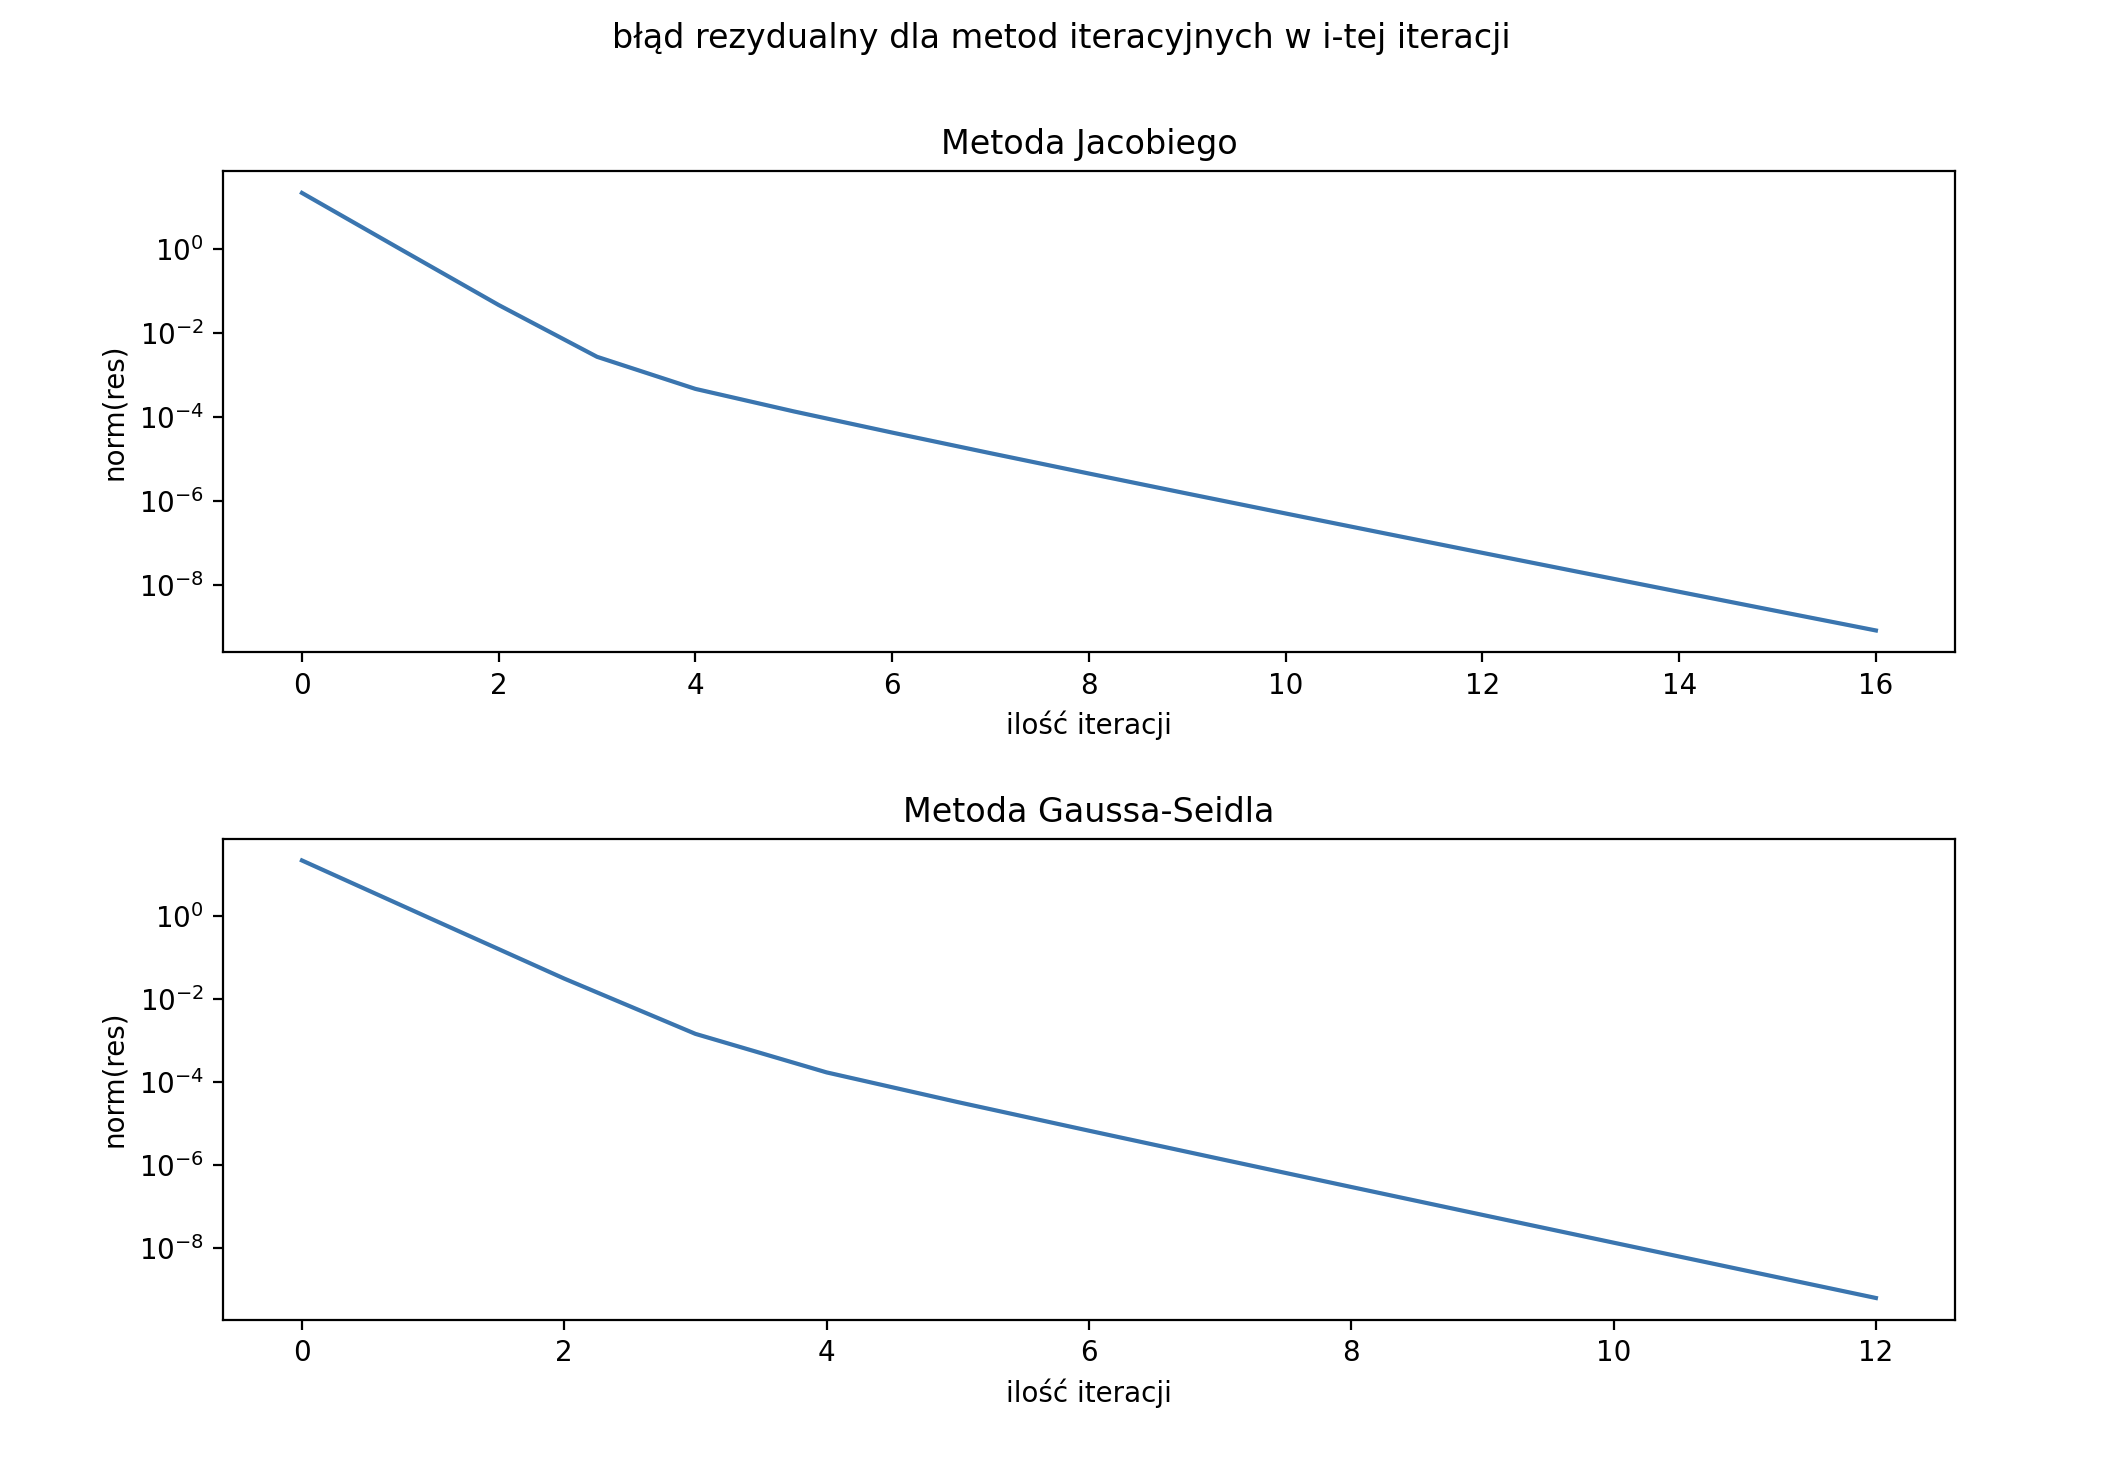
\includegraphics[width=12cm]{z2_residuum}
\end{center}
Zgodnie z wcześniejszymi obserwacjami, metoda Gaussa-Seidla gwarantuje podobne wartości normy wektora residuum parę iteracji wcześniej niż metoda Jacobiego.  W obu przypadkach błędy 
maleją w przybliżeniu wykładniczo (prosta na wykresie w skali logarytmicznej).
\subsection{Metody iteracyjne na zmienionym układzie równań}
Zamieniamy teraz elementy leżące na głównej przekątnej macierzy $\boldsymbol{A}$ na 3.
Macierz nie jest już przekątniowo dominująca zatem nie mamy gwarancji zbieżności metod iteracyjnych.
\begin{center}
	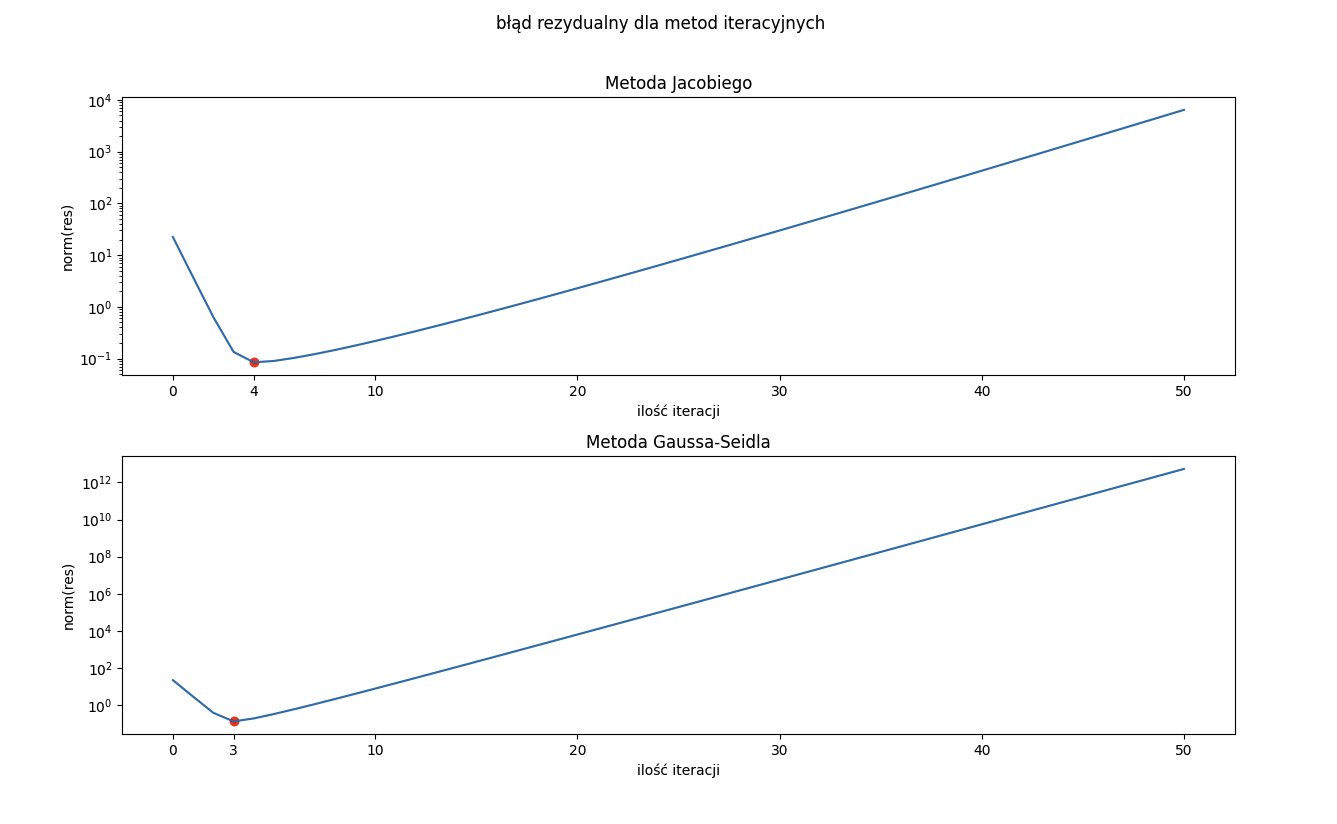
\includegraphics[width=12cm]{z3_residuum}
\end{center}
Rzeczywiście, metody nie zbiegają się. Obie osiągają minimum w okolicach 3,4 iteracji a następnie
wartość błędu rezydualnego zaczyna wzrastać wykładniczo. Obie metody nie są zatem uniwersalne
i mogą nigdy nie osiągnąć wyniku o oczekiwanej dokładności. Warto zwrócić uwagę na to, że
metoda Gaussa-Seidla rozbiega się szybciej niż Jacobiego.

\subsection{Działanie faktoryzacji LU dla zmienionego układu równań}
W przeciwieństwie do metod iteracyjnych, rozwiązywanie układu równań metodą bezpośrednią prowadzi
do znalezienia dokładnego wyniku: 
\begin{center}
\begin{tabular}{ c | c c}
 metoda & czas [ms] & $norm(res)$ \\ 
\hline
 LU & 33038 & $1,03 \cdot 10^{-13}$\\  
\end{tabular}
\end{center}
Rozważane w poprzednim podpunkcie metody, choć pozwalają na szybsze 
znalezienie rozwiązania układu równań o określonej dokładności, 
w pesymistycznym przypadku się rozbiegają, co ogranicza ich stosowalność.
Cechy tej nie ma faktoryzacja LU, natomiast płaci się za to wzrostem złożoności obliczeniowej.
\subsection{Zależności czasu działania metod od rozmiaru macierzy}
Pomiary czasu wykonania algorytmów wykonano dla macierzy o $N \in \{100,500, 1000, 1500, 2000\}$.
\begin{center}
	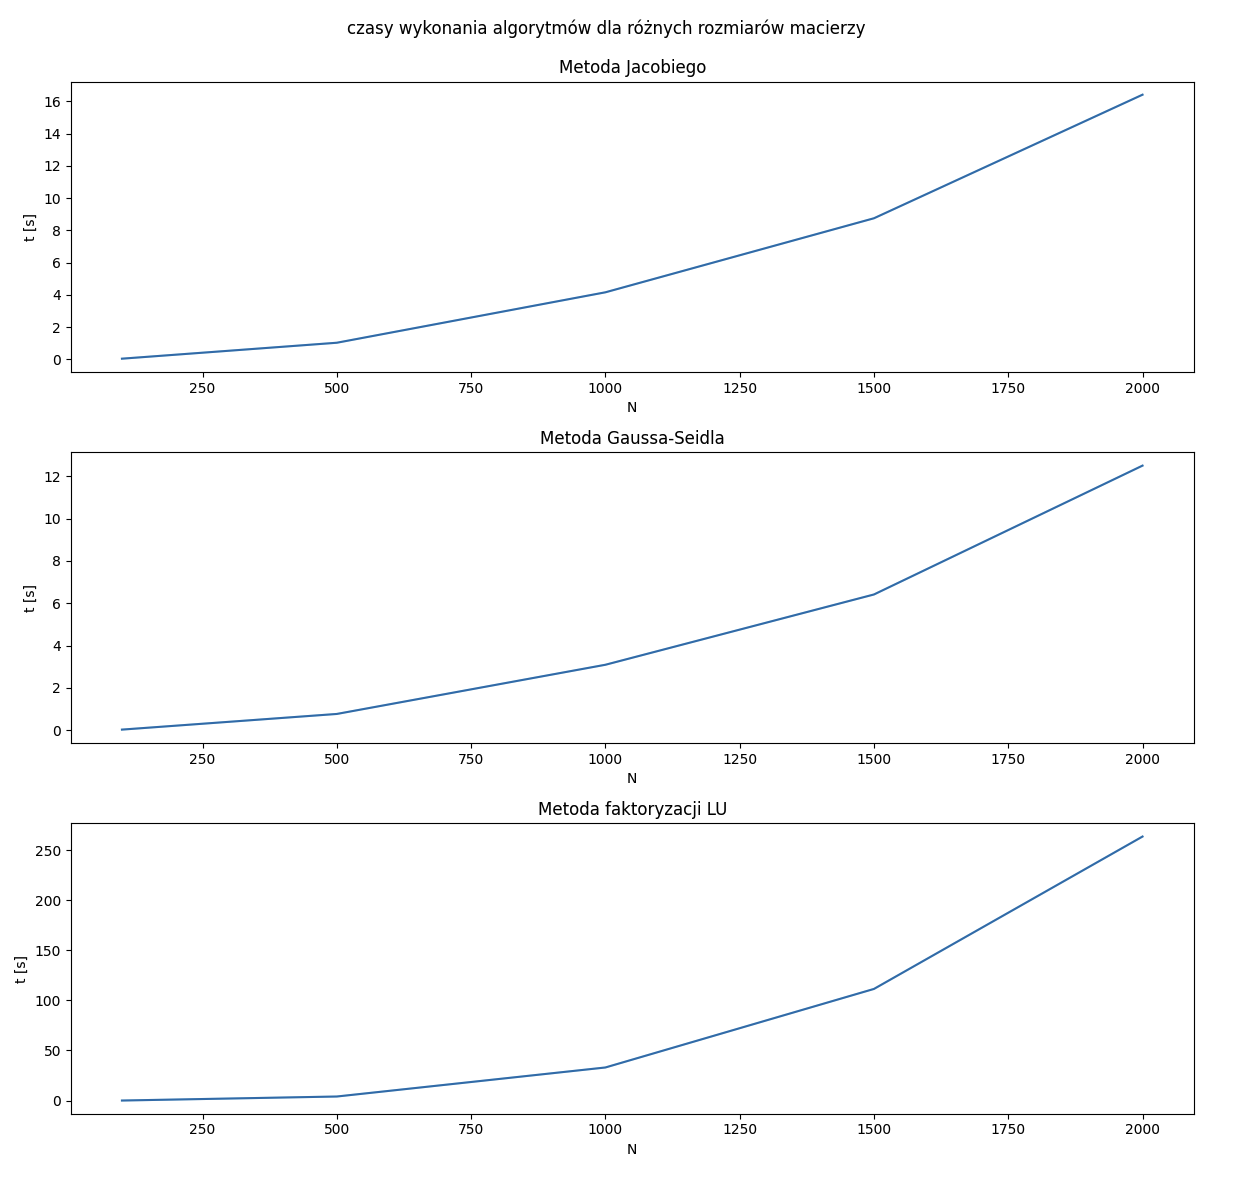
\includegraphics[width=12cm]{z5_czasy}
\end{center}
Na powyższym wykresie potwierdzają się wcześniej postawione hipotezy. Metoda Gaussa-Seidla
charakteryzuje się szybszym wykonaniem od metody Jacobiego,  dla mniejszych $N$ pierwsza metoda
jest mniej więcej półtorakrotnie wolniejsza chociaż wraz ze wzrostem rozmiarów macierzy różnice
czasu wykonania ustalają się na poziomie kilku sekund. Obie metody wykonują się szybciej
od metody faktoryzacji LU, której czas wykonania 
zgodnie z oczekiwaniami rośnie proporcjonalnie do $N^3$ 
(np. dla $N=2000$ wykonuje się ok. 8-krotnie dłużej niż dla $N=1000$).
\begin{center}
	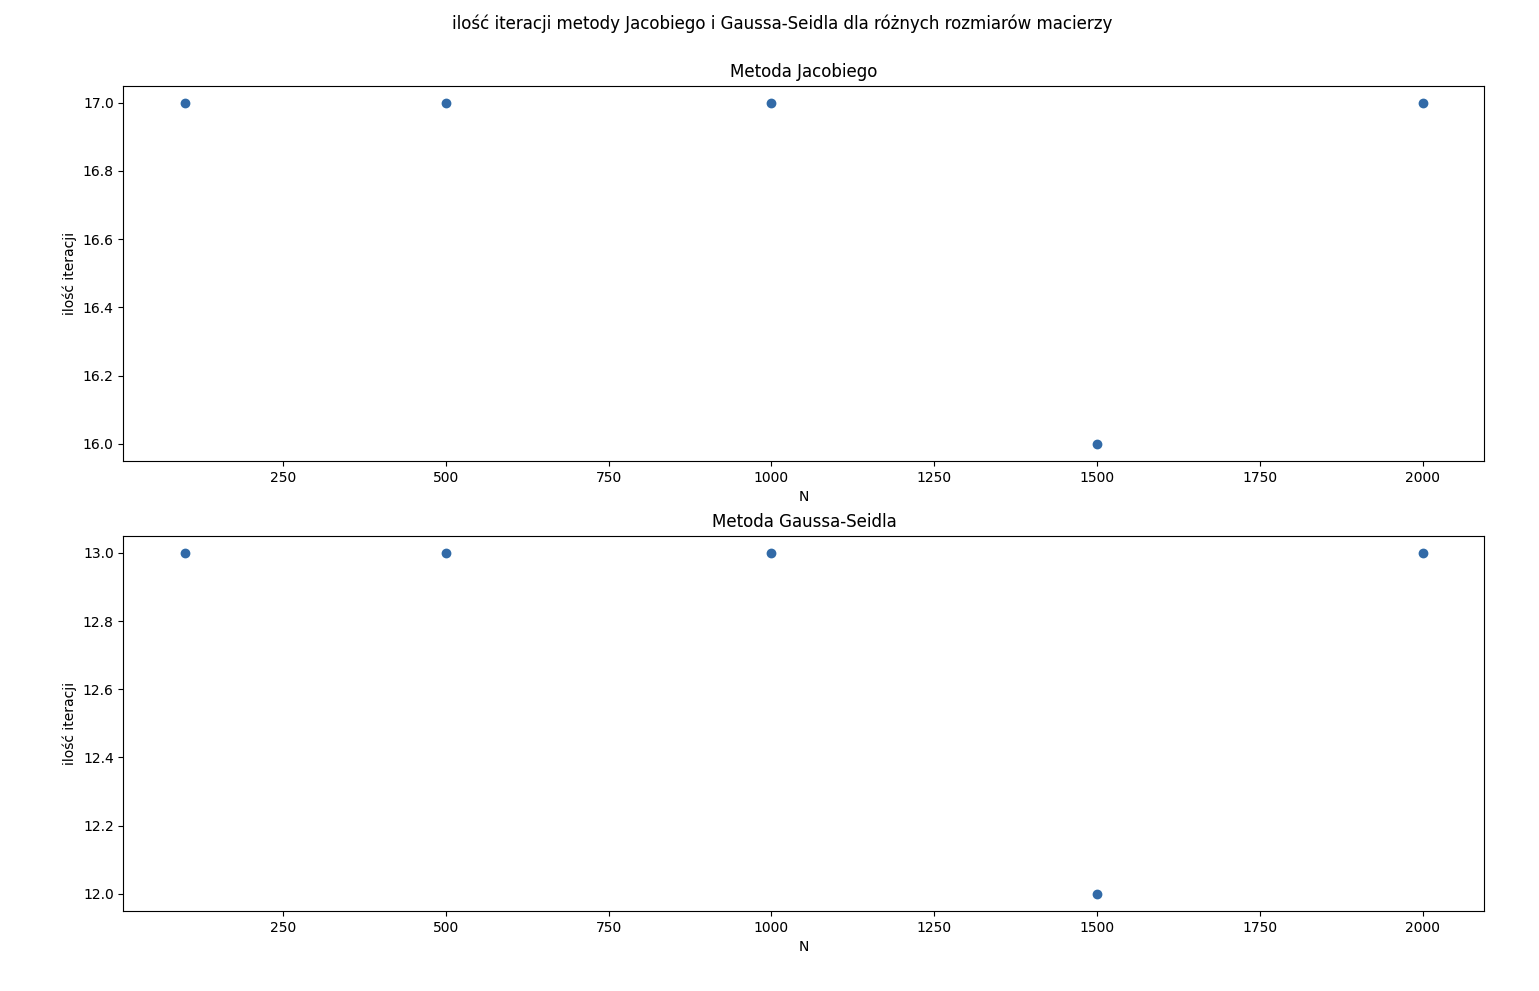
\includegraphics[width=12cm]{z5_iteracje}
\end{center}
Z powyższego wykresu wynika, że rozmiar konstruowanej macierzy pasmowej nie ma większego
wpływu na ilość iteracji metod Gaussa-Seidla i Jacobiego (natomiast pojedyncze iteracje są dłuższe).  Ilość potrzebnych iteracji jest natomiast
związana z oczekiwaną precyzją wyniku, co zilustrowano poniżej.
\begin{center}
	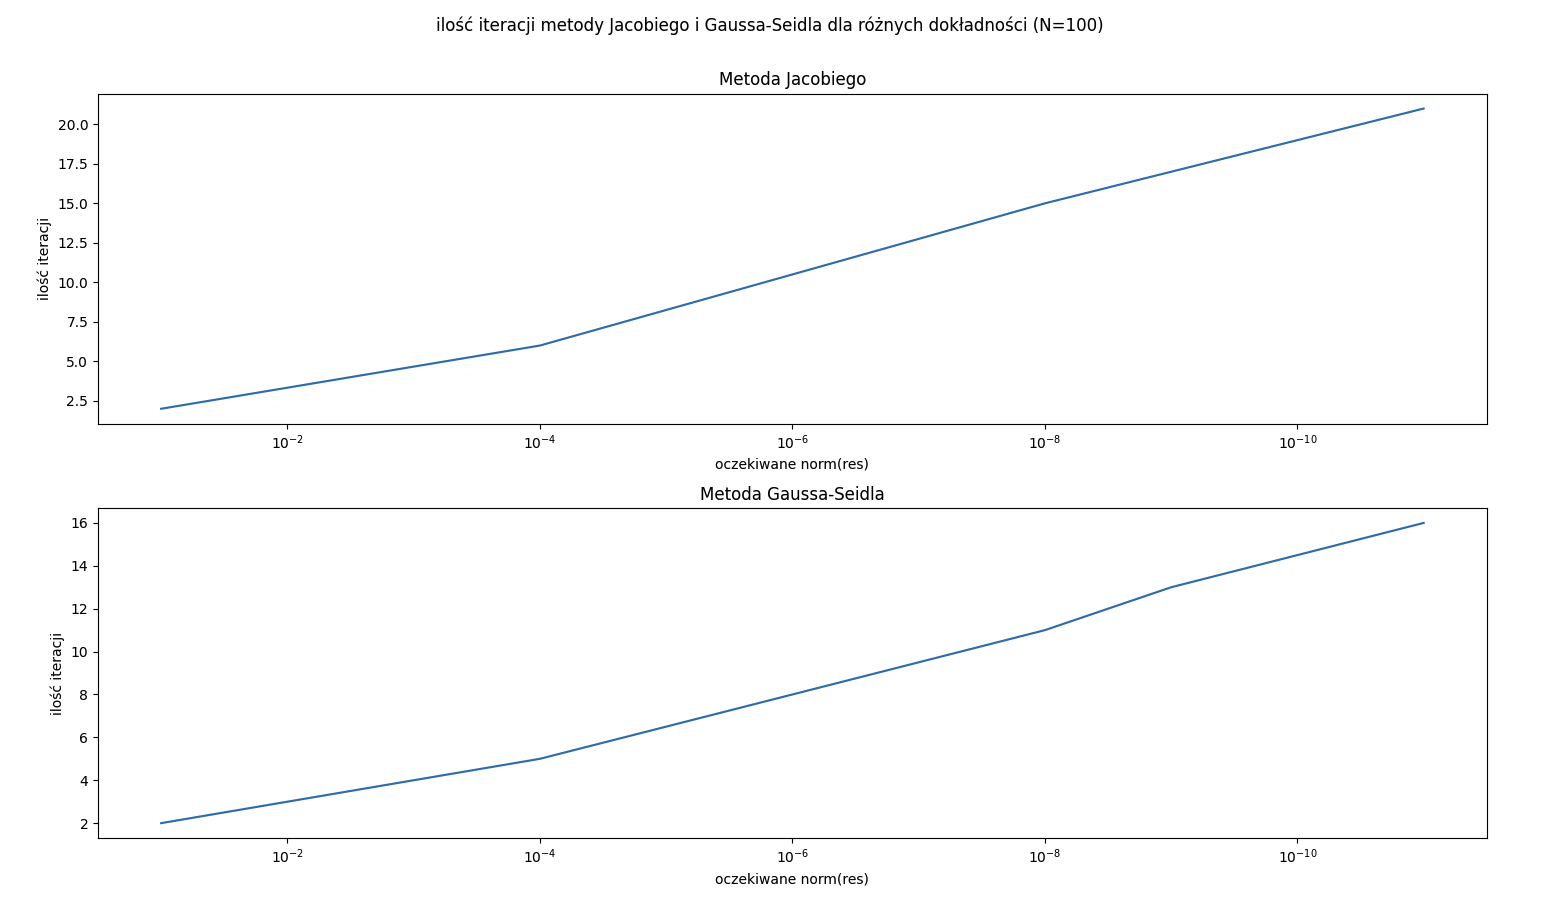
\includegraphics[width=12cm]{z5_oczekiwane_res}
\end{center}

\section{Podsumowanie}
Reasumując, chociaż metoda faktoryzacji LU daje dokładne wyniki, dzieje się to kosztem wysokiej
złożoności obliczeniowej, dla większych macierzy bardziej opłaca się użyć którejś z metod iteracyjnych.
Z drugiej strony, jak wykazaliśmy, metody iteracyjne mogą zawodzić i rozbiegać się.  W analizowanych
przypadkach metoda Gaussa-Seidla okazywała się być szybsza od metody Jacobiego, co związane
było z szybszym zbieganiem się do oczekiwanej złożoności. Nalezy jednak zwrócić uwagę, że w 
wypadku rozbieżności, metoda Gaussa-Seidla szybciej osiągała bardzo wysokie wartości błędu 
rezydualnego.
\section{Źródła}
\begin{itemize}
	\item \href{https://en.wikipedia.org/wiki/Jacobi_method}{Wikipedia-Jacobi}
	\item \href{https://pl.wikipedia.org/wiki/Macierz_przek%C4%85tniowo_dominuj%C4%85ca}{Macierz-
przekatniowo-dominujaca}
\end{itemize}



\end{document}


